\chapter{Preliminares}\label{chapter:REV-LL}

Con este trabajo se persigue diseñar un mecanismo para convertir el espacio discreto de soluciones de un VRP en un espacio de soluciones continuo. Para ello, se presentan en este capítulo los elementos fundamentales de la investigación realizada: los problemas de enrutamiento de vehículos, y las técnicas de ML que se pueden usar para obtener un espacio de soluciones continuo, a partir de soluciones discretas. 


%En este capítulo se presentan un conjunto de técnicas y modelos del aprendizaje automático que han sido empleadas para resolver problemas de enrutamiento. En particular, se enfatiza en aquellas cuya idea central es lograr un mecanismo de codificación y decodificación donde los vectores codificados son usados para conformar un espacio de búsqueda a nuevas soluciones, y además, evidenciar la importancia de los vectores codificados para la generación de nuevos vectores o soluciones. 

%Dentro de ellas se encuentran los \textit{autoencoders} (AEC), un tipo de redes neuronales usados para aprender codificaciones eficientes de los datos y que constituyen el punto de partida para la solución ofrecida en el trabajo. La misma se compone por dos modelos diferentes, el primero de ellos sigue los conceptos de un \textit{autoencoder} clásico, y el segundo, se establece bajo los conceptos de un \textit{variational autoencoder} (VAE), un tipo de \textit{autoencoder} más avanzado \textit{Chollet et al.} \cite{Chollet}. Dicho esto, resulta necesario incluir la teoría y funcionamiento detrás de estos modelos para poder comprender los fundamentos de la solución. 

Primeramente se comienza con una visión general del problema de enrutamiento de vehículos (VRP) y algunas de sus variantes con la sección \ref{2-VRPintro}. En este contexto, se analizan varias formas de representar vectorialmente una solución a una instancia del VRP.

 Luego, en las secciones \ref{2-AEC} y \ref{2-VAE} se expone la teoría y principios detrás de los modelos \textit{autoencoder} (AEC) y \textit{variational autoencoder} (VAE) respectivamente. Ambos modelos son implementados como parte de la solución. También se señalan  algunas aplicaciones de los VAEs a problemas similares a este trabajo.

 Las secciones \ref{2-Seq2seq} y \ref{2-RL} ofrecen varias propuestas existentes en el estado del arte y que, hasta el momento, resultan atractivas en el área del aprendizaje automático para la codificación de secuencias y solución del VRP con heurísticas aprendidas gracias a este tipo de algoritmos. La primera de ellas, aborda las arquitecturas nombradas como \textit{sequence-to-sequence}, muy útiles para tareas donde se requiera transformar de una secuencia a otra.  El acercamiento hacia estas arquitecturas parte de la interpretación que se le puede dar a una solución del VRP como un conjunto de secuencias de clientes. Mientras que la segunda reseña el empleo de \textit{reinforcement learning} \ref{1-RL} en problemas de optimización de tal complejidad, principalmente en el aprendizaje automático de heurísticas para resolver problemas de enrutamiento. 




%para comprender la solución propuesta y las existentes en el estado del arte del problema en cuestión. Principalmente, se enfatiza en los modelos del tipo \textit{encoder-decoder} cuya idea constituye la esencia del objetivo de la tesis. Primero se comienza con una visión general del problema VRP y algunas de sus variantes, para luego dar paso a la teoría de \textit{Autoencoders} y sus aplicaciones en problemas de enrutamiento.

%Luego de haber examinado una introducción al aprendizaje automático es necesario destacar que los avances en este campo han permitido a las redes neuronales realizar una amplia variedad de tareas, entre ellas resolver problemas de optimización combinatoria. La mayoría de estos problemas, incluyendo el VRP, son difíciles de solucionar, desde un punto de vista teórico por ser NP-Duro, y desde un punto de vista práctico por lo costoso que resultan las técnicas computacionales aplicadas. Se han examinado dos líneas principales por parte de la comunidad de ML, una de ellas con el fin de reemplazar el excesivo cómputo por una rápida aproximación; mientras que la otra se basa en explorar el espacio de búsqueda y aprender nuevas heurísticas. En efecto, el empleo de \textit{deep reinforcement learning} ha devenido en un gran interés para aprender heurísticas automáticamente en problemas de tal complejidad. 

%Los problemas de enrutamiento como el TSP y el VRP, se sitúan entre los problemas de optimización más estudiados y con mayores intentos de solución en la práctica.  La aplicación de redes neuronales para optimizar decisiones en problemas de optimización combinatoria se remonta a \textit{Hopfield et al.} \cite{Hopfield1982}; llegando a resolver pequeñas instancias del TSP de hasta 30 ciudades. El desarrollo de arquitecturas de redes neuronales ha allanado el camino a enfoques competitivos basados en ML no solo para dar solución a problemas de enrutamiento, sino también para inspeccionar el espacio de búsqueda continuo que conforman un conjunto de soluciones.





%\newpage

\section{Problema de Enrutamiento de Vehículos}\label{2-VRPintro}

Una solución del VRP requiere la determinación de un conjunto de rutas donde cada una se realiza por un solo vehículo. Las rutas comienzan y terminan en el depósito y están conformadas por una secuencia de clientes que deben ser visitados en ese el orden. La disposición de los clientes dentro del conjunto de rutas debe cumplir con las limitaciones de la flota y restricciones de los clientes, y además, minimizar el costo de transportación u otro criterio \cite{PaoloVigo}.

En un gran número de problemas derivados del VRP se asume que la mercancía a distribuir y la flota de vehículos se encuentran inicialmente en los depósitos. La cantidad de depósitos así como su capacidad para atender a todos o solo a un subconjunto de los clientes determinan las estrategias a seguir en la planificación de las rutas.

Los clientes contienen toda la información relativa al servicio que solicitan. Pueden estar caracterizados por la cantidad y tipo de mercancía que requieren, horarios de atención y tipos de servicios. 

Por lo general, se denota por $V = \{1, 2, ..., n\}$ el conjunto de clientes, $ V^{+} = \{0\} \cup V$ el conjunto formado por los clientes y el depósito $0$, $d_i$ la demanda asociada a cada cliente de $V$ y la flota de vehículos $K = \{1, ..., m\}$, cada uno con capacidad $Q$ . Luego para cada par de elementos $i, j \in V^{+}$ se define el arco $(i, j)$ con el costo del viaje asociado $c_{ij}$ , siendo $C$ la matriz de costos tal que $C[i, j] = c_ij$. Las características de cada problema determinan el concepto de costo y factibilidad de las rutas.

En formulaciones más simples, el costo de una ruta se calcula a partir de la suma de los costos de los arcos involucrados en la misma; también, se asume que la flota la componen vehículos idénticos de capacidad $Q$ y en algunos casos se supone que su número es ilimitado \cite{PaoloVigo}. En problemas más complejos, la flota puede estar compuesta por vehículos diferentes en cuanto a su capacidad, costo fijo y/o variable, longitud máxima de los recorridos que pueden realizar, disponibilidad, etc... \cite{PaoloVigo}. 

Atendiendo a las restricciones que se consideran, los problemas de enrutamiento de vehículos se agrupan en:

\begin{description}
	\item [VRP con restricciones de capacidad (CVRP)] es la variante más estudiada hasta la actualidad según Toth y Vigo en \cite{PaoloVigo}. Todos los vehículos de la flota son idénticos y con capacidad limitada, por lo que durante el recorrido no se debe exceder la capacidad de ninguno de ellos. 
	\item [VRP con flota heterogénea (HVRP)] la flota de vehículos no es homogénea, pues pueden presentar diferentes características. 
	\item [VRP con múltiples depósitos (MDVRP)] existen varios depósitos desde los cuales pueden comenzar y terminar las rutas. La determinación de los depósitos de partida y fin del recorrido son también parte de la solución del problema.
	\item [VRP con ventanas de tiempo (VRPTW)] es una extensión del CVRP \cite{PaoloVigo} donde además de la restricción de capacidad, los clientes establecen un horario conocido como ventana de tiempo en el cual se realizará el servicio. 
	\item [VRP con recogida y entrega (VRPPD)] los clientes solicitan el servicio de recogida y/o entrega de mercancía. 
\end{description}

El \textbf{objetivo de un VRP} es minimizar o maximizar determinada función. Según las características del problema las funciones objetivo  más frecuentes son:
\begin{itemize}
	\item Minimizar el costo de transportación a partir de la distancia recorrida.
	\item Minimizar la cantidad de vehículos.
	\item Minimizar los costos totales, incluidos los costos fijos y los costos variables.
	%\item Optimización jerárquica de la función objetivo: el número de vehículos es el objetivo principal de optimización, y luego se optimizará la distancia de viaje del vehículo correspondiente.
\end{itemize}


Las funciones objetivo se evalúan a partir de las soluciones candidatas del problema de enrutamiento. La determinación de una representación vectorial adecuada para las soluciones, resulta una decisión importante en este tipo de tareas. Es por ello que en las próximas secciones se exponen tres formas diferentes de lograrlo

\subsection{Representación de soluciones del VRP}\label{2-solS}

Una \textbf{solución para el VRP} (en su versión más simple) es un conjunto de listas de clientes, donde cada lista representa una ruta. Por ejemplo:


\begin{equation}
\label{s8}
s = [(2, 5, 1), (6, 4), (7, 8, 3)],
\end{equation}

representaría una solución con tres rutas para una instancia del problema con 8 clientes. En la primera se va desde el depósito hasta el cliente 2, de ahí al 5, después al 1, y por último se regresa al depósito. La segunda ruta parte del depósito, se visitan los clientes 6 y 4, en ese orden, y se regresa al depósito. Para la tercera es similar, el recorrido inicia en el depósito y luego son visitados los clientes 7, 8 y 3, respetando el orden, y finalmente se retorna al depósito. Luego, las soluciones a problemas de $n$ clientes estarían dadas por listas de este estilo con dígitos entre 1 y $n$. 

Sin embargo, si en $s$ se intercambia el orden de las dos últimas rutas como se observa en \ref{s8p}:

\begin{equation}
\label{s8p}
s_1= [(2, 5, 1), (7, 8, 3), (6, 4)],
\end{equation}
 
el resultado constituye la misma solución, pues el orden dentro del conjunto de rutas no afecta el costo y las rutas como tal no cambiaron. Debido a ello, las permutaciones entre las rutas conducirán a la misma solución. 

Para evitar estas repeticiones, en este trabajo se asumirá que todas las permutaciones a partir de una solución $s$ son iguales. Para ello se considera ordenar las rutas según el primer elemento o cliente de la ruta. Por ejemplo, la solución vista inicialmente en \ref{s8} representaría a todas las siguientes:


\begin{eqnarray*}
s &=&  [(2, 5, 1), (6, 4), (7, 8, 3)],\\
s_1 &=& [(2, 5, 1), (7, 8, 3), (6, 4)],\\
s_2 &=& [(7, 8, 3), (2, 5, 1), (6, 4)],\\
s_2 &=& [(7, 8, 3), (6, 4), (2, 5, 1)],\\
s_3 &=& [(6, 4), (7, 8, 3), (2, 5, 1)],\\
s_4 &=& [(6, 4), (2, 5, 1), (7, 8, 3)].\\
\end{eqnarray*}

Obtener una representación continua de las soluciones anteriores forma parte del objetivo de este trabajo. Para resolverlo, se usó un modelo de redes neuronales cuyo funcionamiento es posible mediante operaciones vectoriales. No obstante, como se mencionó en \ref{1-etapas}, los datos deben cumplir ciertas características como la normalización. 

Con este fin, se abordan en este trabajo, otros dos tipos de representaciones vectoriales de gran utilidad para el modelo propuesto. La primera de ellas mediante un vector de números enteros simbolizando la adyacencia entre clientes en un grafo dirigido, y la segunda, a través de una matriz binaria de ceros y unos. Estas representaciones se definen en las secciones \ref{2-Graph} y \ref{2-Matrix} respectivamente. 

\subsection{Representación a través de grafos}\label{2-Graph}

Como se había mencionado en \ref{2-VRPintro}, un problema de enrutamiento de vehículos se caracteriza por un conjunto $V$ de $n$ clientes, una flota $K$ de $m$ vehículos con capacidad $Q$ y una matriz de costos $C$. Una solución de este problema, como la mostrada en \ref{2-solS}, puede ser definida formalmente como un grafo dirigido $G(V,E)$ tal que:

\begin{enumerate}
	\item $V = \{1, 2, ..., n\}$ es el conjunto de vértices del grafo, en correspondencia con los clientes.
	
	\item $E = \{(i, j) | 0 < i, j \leq n, i \neq j \}$ el conjunto de aristas que conforman las rutas. De forma tal que si $(i, j) \in E$ significa que el cliente $j$  se visita después que $i$ en el recorrido.
\end{enumerate}    

Al retomar el ejemplo visto en \ref{2-solS} donde $s = [(2, 5, 1), (6, 4), (7, 8, 3)]$ el grafo correspondiente de 8 vértices quedaría conformado por el siguiente conjunto de aristas: 

\begin{equation}
\label{2-Es8}
	E = \{(2, 5), (5, 1), (6, 4), (7, 8), (8, 3)\}
\end{equation}

Gráficamente las componentes del mismo simbolizan a cada una de las rutas como se observa a continuación:

\begin{center}
	$2 \rightarrow 5 \rightarrow 1$\\
	$6 \rightarrow 4$ \\
	$7 \rightarrow 8 \rightarrow 3$\\	
\end{center}

A partir de $G$ se puede obtener una representación vectorial de una solución mediante un vector de longitud $n$. Dicho vector será denotado como $p$ y constituye un vector de adyacencias entre los clientes en las rutas. De forma tal que $p[j] = i$ si $i + 1$ es el padre de $j + 1$ en el grafo, es decir, el cliente $i + 1$ es el antecesor del cliente $j + 1$ en la ruta a la que pertenecen.

Por ejemplo, en el conjunto de aristas \ref{2-Es8}, la arista $(2, 5)$ significa que el cliente $5$ es visitado después del cliente $2$; de la misma forma para la arista $(8, 3)$, donde el cliente $3$ es quien le sigue al $8$ en el recorrido. Por lo tanto, para estos dos casos se tendría que $p[4] = 1$  y $p[2] = 7$ respectivamente.

 Entonces $p$ cumple lo siguiente:

\[p[j]=\left\{
\begin{array}{rcl}
\label{2-pi}
i & \mbox{si} & \text{el cliente $j + 1$ va detrás de $i + 1$ en la ruta}\\
&
& \\
j & \mbox{si} & \text{si $j + 1$ es comienzo de ruta }  \\
&
& \\
\end{array}
\right. \]

Luego para obtener el vector $p$ correspondiente a $s$ es necesario tener en cuenta las relaciones de adyacencia establecidas en $E$. El procedimiento consiste en tomar cada arista $(i, j) \in E$ interpretada como: $j$ es el cliente que está a continuación de $i$ en su ruta, y fijar $p[j - 1] = i - 1$. Cada uno de los pasos para el ejemplo \ref{2-Es8} se enumeran a continuación:

\begin{eqnarray*}
	(2, 5) & \rightarrow & p[5 - 1] = 2 - 1  \rightarrow p[4] = 1\\
	(5, 1) & \rightarrow & p[1 - 1] = 5 - 1  \rightarrow p[0] = 4\\
	(6, 4) & \rightarrow & p[4 - 1] = 6 - 1  \rightarrow p[3] = 5\\
	(7, 8) & \rightarrow & p[8 - 1] = 7 - 1  \rightarrow p[7] = 6\\
	(8, 3) & \rightarrow & p[3 - 1] = 8 - 1  \rightarrow p[2] = 7\\
\end{eqnarray*}

Además se deben añadir los casos pertinentes a los inicios de rutas: 2, 6, y 7, bajo la condición de que si el cliente $j + 1$ es comienzo de una ruta entonces se cumple que $p[j] = j$. Al aplicar esta definición se obtiene:

\begin{eqnarray*}
	2 & \rightarrow & p [2 - 1] = 2 - 1 \rightarrow p[1] = 1\\
	6 & \rightarrow & p [6 - 1] = 6 - 1 \rightarrow p[5] = 5\\
	7 & \rightarrow & p[7 - 1] = 7 - 1  \rightarrow p[6] = 6\\
\end{eqnarray*}
Finalmente el vector $p$ resulta en $[4, 1, 7, 5, 1, 5, 6, 6]$.

%TODO: hacer foticos para mostrar el vector con los índices más bonito


Si en $s$ existiera una ruta formada por un solo cliente, por ejemplo un noveno cliente, la nueva solución $s'$ quedaría conformada como:
\begin{equation}
\label{2-s9}
	s' = [(2, 5, 1), (6, 4), (7, 8, 3), (9)]
\end{equation}
 Al intentar determinar su vector $p'$ correspondiente,  entraría en el último caso de análisis donde el cliente es comienzo de ruta. Por tanto, la interpretación se reduce a $p'[9 - 1] = 9-1 \rightarrow p'[8] = 8$. Luego, al adicionarlo al vector se obtiene $p' = [4, 1, 7, 5, 1, 5, 6, 6, 8]$. 
 
 En dependencia de la cantidad de clientes del problema particular, y siguiendo la definición dada en \ref{2-pi}, se pueden generar un número considerable de vectores que las cumplan. En este sentido, la generación de soluciones del VRP resulta más fácil, sin tener que estar ordenando las rutas como en la representación a través de listas de rutas vista en \ref{2-solS}. Por tal motivo, el conjunto de datos iniciales se generó según la representación de soluciones vista en esta sección, o sea, mediante los vectores $p$ asociados a la solución de una instancia del VRP.
 
 No obstante, estos vectores $p$ aún no están normalizados, por tanto, en la siguiente sección se introduce una nueva manera de representar soluciones con la ayuda de matrices binarias. Las mismas juegan un papel fundamental en este trabajo, pues conforman el conjunto de datos conque se entrenó y evaluó la solución ofrecida. 
 
\subsection{Representación de las soluciones mediante matrices binarias}\label{2-Matrix}

Esta otra representación vectorial también se basa en la definición del grafo determinado en \ref{2-Graph}, pero en esta ocasión, mediante una matriz binaria. Se denota como $M$ la matriz binaria de dimensión $nxn$ tal que $M[i, j] \in \{0, 1\} \forall i, j \in \{0, ..., n-1\}$ . Las soluciones al VRP que se representen mediante estos vectores cumplen con la siguiente definición: 

\[M[i, j]=\left\{
\begin{array}{rcl}
\label{2-Mdef}
1 & \mbox{si} & \text{el cliente $j + 1$ va detrás de $i + 1$ en la ruta}\\
&
& \\
1 & \mbox{si} & \text{$i = j$, la ruta está formada por un único cliente i + 1}  \\
&
& \\
0 & \mbox{eoc}.  \\
\end{array}
\right. \]

A partir de la definición anterior se cumplen las siguientes propiedades:
\begin{enumerate}
	\item Si la fila $i-$ésima es completamente nula, entonces el cliente $i+1$ es el último en su ruta.
	\item Si la columna $j-$ésima es nula entonces el cliente $j+1$ es el inicio de la ruta a la que pertenece.
	\item Si $M[i, i] = 1$ es porque el cliente $i + 1$ es el único en su ruta.
\end{enumerate}

Con el fin de visualizar la definición y propiedades anteriores se construirá la matriz correspondiente a la solución del ejemplo \ref{2-s9}, la cual incluye una ruta con un único cliente.
\begin{equation*}
\label{2-s9M}
s' = [(2, 5, 1), (6, 4), (7, 8, 3), (9)].
\end{equation*}
En este caso el conjunto de aristas se conformaba como:
 \begin{equation*}
 \label{2-Es9}
 E = \{(2, 5), (5, 1), (6, 4), (7, 8), (8, 3)\}.
 \end{equation*}
 Al añadir una nueva ruta con un solo cliente no se sumó ninguna otra arista debido a que ese elemento en el grafo no está relacionado con ningún otro.  El proceso de construcción es similar al del vector $p$ en \ref{2-Graph}, por cada arista del grafo se añade el valor correspondiente según la definición. A continuación se muestran los pasos que se deben desarrollar:
 
 \begin{eqnarray*}
 	(2, 5) & \rightarrow & M[1, 4] = 1 \\
 	(5, 1) & \rightarrow & M[4, 0] = 1 \\
 	(6, 4) & \rightarrow & M[5, 3] = 1 \\
 	(7, 8) & \rightarrow & M[6, 7] = 1 \\
 	(8, 3) & \rightarrow & M[7, 2] = 1 \\
 \end{eqnarray*}
 
 En los pasos anteriores, se observa que la posición $(1, 4)$ de $M$ tendrá valor $1$ porque existe la arista $(2, 5)$ en $E$, lo que se traduce a que el cliente 5 va detrás del 2 en la primera ruta de \ref{2-s9M}. De la misma forma ocurre con el resto de las aristas.
  
 Además, con la restricción correspondiente al cliente $9$ por ser el único en su ruta, se tiene que $M[8, 8] = 1$. En este punto, ya se aplicaron las dos primeras condiciones de la definición, solo faltaría adicionar que el resto de las posiciones de la matriz tomarían valor igual a 0. Dicho todo esto, ya $M$ está completamente definida y quedaría conformada como: 
 
 \begin{equation}
 \label{M9}
 \centering
 \begin{pmatrix}
 0 & 0 & 0 & 0 & 0 & 0 & 0 & 0 & 0\\
 0 & 0 & 0 & 0 & 1 & 0 & 0 & 0 & 0\\
 0 & 0 & 0 & 0 & 0 & 0 & 0 & 0 & 0\\
 0 & 0 & 0 & 0 & 0 & 0 & 0 & 0 & 0\\
 1 & 0 & 0 & 0 & 0 & 0 & 0 & 0 & 0\\
 0 & 0 & 0 & 1 & 0 & 0 & 0 & 0 & 0\\
 0 & 0 & 0 & 0 & 0 & 0 & 0 & 1 & 0\\
 0 & 0 & 1 & 0 & 0 & 0 & 0 & 0 & 0\\
 0 & 0 & 0 & 0 & 0 & 0 & 0 & 0 & 1\\
 \end{pmatrix}
 \end{equation}
 
 En la matriz anterior se cumple que las filas con índices $0, 2, 3$ y $8$, correspondientes a los clientes 1, 3, 4 y 9 respectivamente, son completamente nulas de acuerdo a la propiedad número 1. Pues estos clientes, como se observa en \ref{2-s9M}, son los finales de la ruta a la cual pertenecen, o sea, no existe ningún otro cliente que le suceda. 
 
 %En la tercera ruta de $s'$ \ref{2-s9M} el cliente $8$ es visitado después del cliente $3$ y antes que el cliente número 3. Este orden se establece en la matriz $M$  por las posiciones $(6, 7)$ y $(8, 3)$ cuyo valor es 1.
 
  También se tiene que las columnas de índices $1, 5$ y  $6$ pertenecientes a los clientes $2, 6$ y $7$ tienen todos sus valores iguales a cero, como plantea la segunda propiedad. Como el cliente 9 es el único en su ruta, o sea, es inicio y final simultáneamente, según las propiedades lo que debería pasar es que $M[8, 8]$ sea igual a $0$ pero según la definición se fijará con el valor 1. Esta decisión se tomó  para añadir más valores distintos de cero a la matriz, por tanto $M[8, 8] = 1$. 
  
  Una vez representadas las soluciones de un VRP de manera vectorizada y normalizada (con posibles valores 0 o 1) con las matrices $M$, ya se consigue que los datos cumplan con las características requeridas. Por tanto, los conjuntos de datos de entrenamiento, validación y prueba empleados durante los experimentos realizados, se aprovechan de las matrices binarias analizadas previamente.
  
  La conformación del modelo mencionado se abordará en el capítulo \ref{chapter:Solution}, pero antes de llegar a ese punto, es necesario comprender los fundamentos de la arquitectura de redes neuronales seleccionada, conocida como \textit{autoencoder}. En la siguiente sección se da inicio a tal contenido.
 
 
 
\section{Autoencoders}\label{2-AEC}

Muchos algoritmos de aprendizaje profundo no supervisado \ref{1-MLnosupervisado} se basan en la idea de \textit{autoencoders}, según refieren Russell y Norvig en \cite{PeterNorvig} . Estos modelos intentan obtener una representación o código de los datos de entrada de forma tal que la transformación sea provechosa en determinada tarea.

Los \textit{autoencoders} pueden aprender propiedades de los datos sin la necesidad de etiquetas anotadas por humanos, por esta razón es que son clasificados como algoritmos de aprendizaje no supervisado \ref{1-MLnosupervisado}. 

%Ian/499
La idea de los \textit{autoencoders} ha sido parte del panorama histórico de las redes neuronales desde 1980 \cite{LeCun1987, HintonAutoencoders}. Tradicionalmente han sido usados para reducción de dimensión o extracción de características \cite{autoencoders2020, VAESurveyAplications}. Las conexiones teóricas entre los modelos de variable latente y \textit{autoencoders} han ubicado a estos últimos dentro de la familia de modelos generativos. Pueden ser considerados como un caso especial de redes \textit{feedforward} y por lo tanto, ser entrenados con las mismas técnicas de descenso del gradiente y \textit{backpropagation}.

Un \textit{autoencoders} es un modelo que contiene dos partes:
\begin{description}
	\item[Encoder: ]  función $f$ que transforma la entrada $x$ en un vector latente $\hat{z}$ de menor dimensión, $\hat{z} = f(x)$. Como el vector latente es de baja dimensión, el \textit{encoder} se obliga a aprender solo las características más importantes de los datos de entrada. 
	\item[Decoder: ] Trata de reproducir la entrada $\tilde{x}$ a partir del vector latente $\hat{z}$, $\tilde{x} = g(\hat{z})$. Aunque $\hat{z}$ tiene una menor dimensión, posee el tamaño suficiente para permitir al \textit{decoder} recuperar la entrada.
\end{description}
El modelo se entrena de forma tal que $x \approx g(\hat{z})$, o sea, el proceso de codificación sea revertido por el decodificador lo mejor posible. 

Según plantea \textit{Goodfellow et al.} \cite{BengioGood}, para los modelos generativos no resulta conveniente lograr que $g(f(x)) = x$ para todos los valores de la entrada. Esto se debe a que la idea es generar nuevos elementos no conocidos y que pertenezcan a la distribución subyacente en los datos. En cambio, se espera que al entrenar el modelo para que genere la misma entrada, se obtenga una representación capaz de agrupar aspectos y propiedades significativas de los datos \cite{BengioGood}.

 En la figura \ref{AEdiagram} se muestra un esquema general del modelo  \textit{autoencoders} que contiene los elementos antes mencionados:

\begin{figure}[!h]
	
	\centering
	
	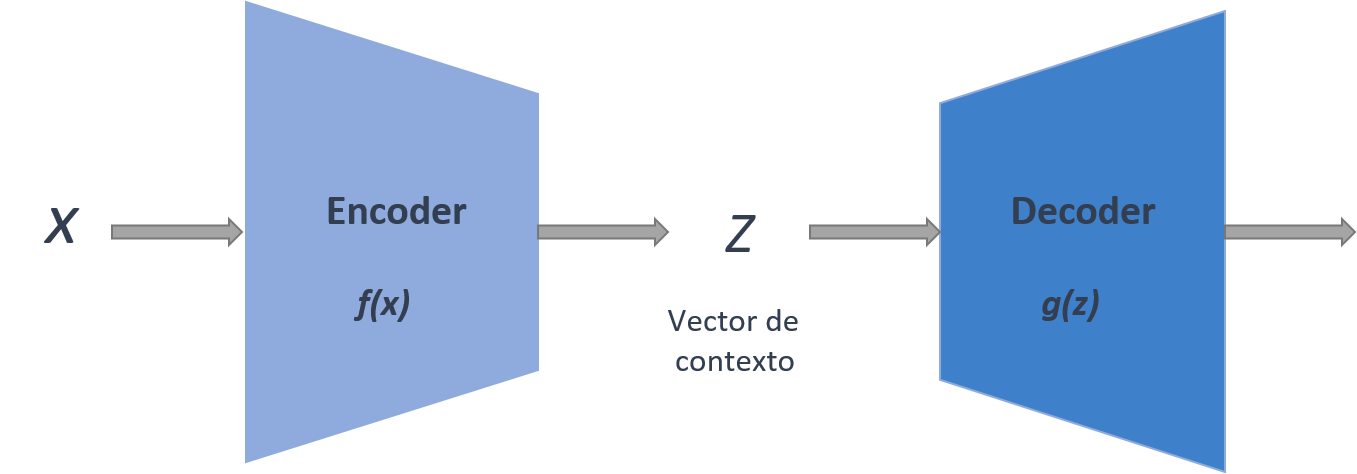
\includegraphics[width=4in]{Graphics/AEdiagram.png}
	
	\caption{\small{Diagrama general de un \textit{autoencoders}}}
	%\url{https://arxiv.org/abs/1802.07228}
	
	\label{AEdiagram}
	
\end{figure}

Un ejemplo de \textit{autoencoders} muy simple es el \textit{autoencoders} lineal, donde $f$ y $g$ son lineales y comparten la matriz de pesos $W$:
\begin{eqnarray*}
	\hat{z} &=& f(x) = Wx \\
	\tilde{x} &=& g(\hat{z}) = W^{\top}\hat{z}.
\end{eqnarray*}

El proceso de aprendizaje se describe como minimizar una función
\begin{equation}
	\mathcal{L}(x, g(f(x))),
\end{equation}
donde $	\mathcal{L}$ es una función de pérdida que penaliza a $g(f(x))$ por ser diferente de $x$. Un ejemplo sería calculando el error cuadrático medio
\begin{equation*}
\mathcal{L}	= \sum_{j}\parallel x_j - g(f(x_j)) \parallel^{2}.
\end{equation*}

\begin{figure}[!h]
	
	\centering
	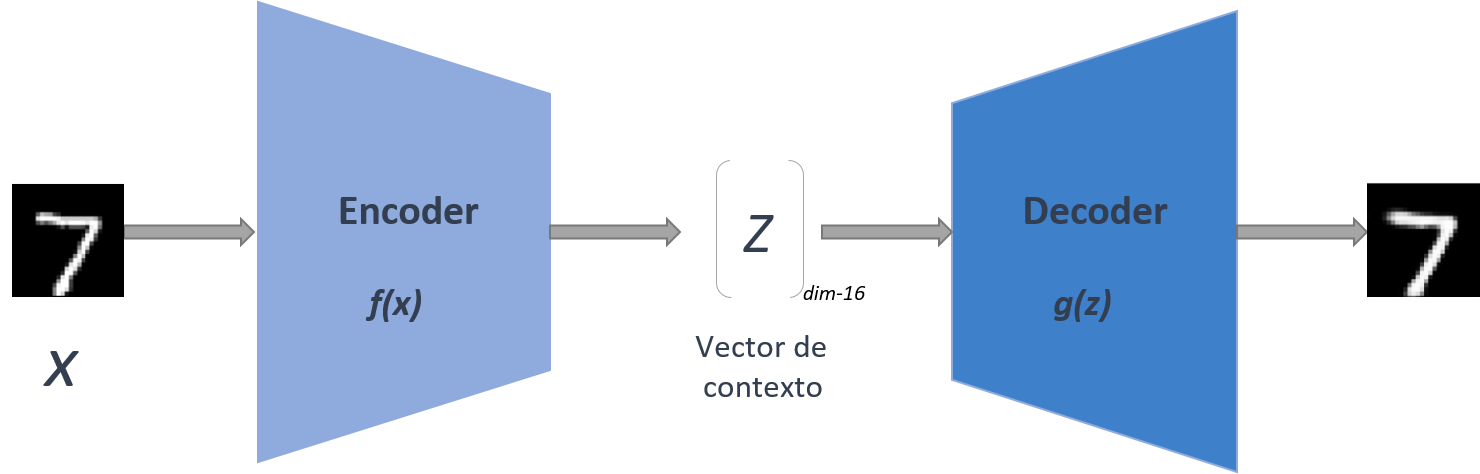
\includegraphics[width=4in]{Graphics/AEMnist.png}
	
	\caption{\small{Un \textit{autoencoders} con dígitos de MNIST como entrada y salida. El espacio latente es de dimensión 16. MNIST es una base de datos de imágenes con dígitos del 0 al 9 escritos a mano.}}
	
	\label{AEminist}

	
\end{figure}

Si la entrada se trata como una distribución, se puede interpretar el \textit{encoder} como un codificador de la distribución $p(z|x)$, y el \textit{decoder}, como un decodificador de la distribución $p(x|z)$. La función de pérdida del \textit{autoencoders} se expresa como:
\begin{equation}
	\mathcal{L} = - \log p(x|z).
\end{equation}

Si se asume que la distribución de la salida del \textit{decoder} es Normal, entonces la función de pérdida se traduce en:
\begin{equation}
	\label{GaussLoss}
	\mathcal{L} = -\log p(x|z) = -\log \prod_{i = 1}^{m}\mathcal{N}(x_i, \tilde{x_i}, \sigma^{2}) = -\sum_{i=1}^{m}\log\mathcal{N}(x_i, \tilde{x_i}, \sigma^{2})\alpha\sum_{i = 1}^{m}(x_i - \tilde{x_i})^{2}.
\end{equation}
En la ecuación \ref{GaussLoss}, $\mathcal{N}(x_i, \tilde{x_i}, \sigma^{2})$ representa una distribución Normal con media $\tilde{x_i}$ y varianza $\sigma^{2}$, siendo esta última constante. La salida del \textit{decoder} $\tilde{x_i}$ se asume independiente y de dimensión $m$.

 Los \textit{autoencoders} se aplican a muchos problemas, desde el reconocimiento facial \cite{zeng2018facial, chen2018softmax}, detección de características \cite{masci2011stacked, rifai2011contractive}, detección de anomalías \cite{zhou2017anomaly, sakurada2014anomaly}, traducción automática \cite{BahdanauAlignTrans, SutskeverSeq2seqNN} hasta generar aleatoriamente nuevos datos que son similares a los datos de entrada o de entrenamiento.
 
Algunos ejemplos de estos modelos son los \textit{ autoencoders} regularizados que son efectivos en el aprendizaje de representaciones para tareas de clasificación \cite{AECClasif} y los \textit{variational autoencoders}, con aplicaciones como modelos generativos \cite{VAESurveyAplications, HottungBT21}. En las siguientes secciones se presentarán estos modelos.

\subsection{ Autoencoders regularizados}\label{2-RegAEC}

 Dado que se desea que el modelo descubra atributos latentes dentro de los datos, es importante asegurar que el \textit{autoencoder} no esté aprendiendo simplemente una forma eficiente de memorizar los datos de entrenamiento. Existen varias técnicas de regularización de la red neuronal con el objetivo de garantizar buenas propiedades de generalización \cite{BengioGood, Advanced}. 

Los \textit{autoencoders} regularizados, en lugar de limitar la capacidad del modelo manteniendo una arquitectura poco profunda del \textit{encoder} y \textit{decoder} , así como una reducción de dimensión forzada, utilizan una función de pérdida para alentar al modelo a asumir propiedades que van más allá de la simple capacidad de copiar la entrada en la salida \cite{BengioGood}. 

 %Entre estas propiedades se puede mencionar la dispersión en la capa de representación, valores muy pequeños de la derivada del vector latente y manejo del ruido o falta de información en las entradas.

%Un \textbf{\textit{sparse autoencoder(SAE)}} es simplemente un \textit{autoencoders} cuyo criterio de aprendizaje envuelve una función de penalidad $\Omega(z)$ sobre la dispersión de la capa de código o codificación $\hat{z}$ en conjunto con el error de reconstrucción.
%\begin{equation}
	%\mathcal{L}(x, \tilde{x}) + \Omega(\hat{z})
%\end{equation}
%Estos modelos son típicamente usados para aprender particularidades en otro tipo de tareas como la clasificación. La idea intuitiva detrás de los mismos es forzarlo a activar algunas regiones de la red selectivamente en dependencia de los datos de entrada, de manera que sean extraídas la mayor cantidad de peculiaridades o al menos las más importantes.

%Existen dos formas de imponer la restricción de dispersión; ambas implican medir las activaciones de la capa oculta para cada \textit{batch} de entrenamiento y añadir algún término a la función de pérdida con el fin de penalizar excesivas activaciones. Estos términos son:
%\begin{itemize}
	%\item \textbf{Regularización L1:} penaliza el valor absoluto del vector de activaciones $a$ en la capa $\hat{z}$ para la observación $i$, escalado por un parámetro de ajuste $\lambda$.
	%\begin{equation}
	%	\mathcal{L}(x, \tilde{x}) + \lambda\sum_{i}|a_i^{(\hat{z})}|
	%\end{equation}
	%\item \textbf{Divergencia de Kullback-Leibler  (KL):} en esencia es una medida no simétrica de similitud o diferencia entre dos funciones de distribución de probabilidad. Se define a $\rho$ como un parámetro de dispersión, el cual denota el promedio de activación de una neurona sobre una colección de observaciones. Su valor puede ser aproximado mediante la fórmula $\hat{\rho_j} = \frac{1}{m} \sum_{i}[ a_i^{(\hat{z})}(x)]$ donde el subíndice $j$ denota una neurona específica en la capa $\hat{z}$, y $m$ la cantidad de observaciones $x$. Finalmente el término agregado resulta en:
	%\begin{equation}
	%	\mathcal{L}(x, \tilde{x}) + \sum_{j}KL(\rho||\hat{\rho_j})
	%\end{equation}
	%siendo $\rho$ la distribución idealmente presente en las observaciones de los nodos de la capa oculta. 
%\end{itemize}

%Otro enfoque para desarrollar un modelo generalizable es corromper ligeramente los datos de entrada, o sea, añadirle ruido a la información, manteniendo los datos originales como objetivo. Conocidos como \textbf{\textit{denoising autoencoders(DAE)}} se orientan a minimizar la función  $\mathcal{L}(x, g(f(\tilde{x}))$ donde $\tilde{x}$ es una copia de $x$ alterada por alguna variante de ruido. Esta técnica garantiza que el modelo no pueda simplemente desarrollar un mapeo que memorice los datos de entrenamiento porque en esta versión no son iguales la entrada y la salida.

Se esperaría que para entradas muy similares, la codificación aprendida también fuera muy similar. En otras palabras, que para pequeños cambios en la entrada, se mantenga un estado codificado muy similar. La estrategia de regularización que se conoce como  \textbf{\textit{contractive autoencoders}} está basada en esta idea. 
%Su idea es bastante parecida a un \textit{denoising autoencoders } en el sentido de que esas pequeñas perturbaciones en la entrada pueden considerarse ruido y se desea que el modelo sea robusto ante las mismas.
En ellas se penalizan las instancias donde un pequeño cambio en la entrada conduce a un gran cambio en el espacio de codificación.  

La nueva función de pérdida, además de contar con la pérdida de reconstrucción intrínseca en el entrenamiento, se le adiciona un término de penalización denotado como $\Omega(\hat{z}, x)$ que se relaciona con la entrada $x$ y el vector de codificación $\hat{z}$. 

En los \textit{contractive autoencoders}, este término corresponde a la norma de Frobenius de la matriz jacobiana del vector de codificación $\hat{z}$ con respecto a la entrada. La norma de Frobenius es una generalización de la norma Euclidiana y en este caso el regularizador tiene la forma $\lambda\sum_{i} \parallel \nabla_{x} \hat{z_i}\parallel^{2}$. Luego la función de pérdida resulta en:

\begin{equation}
\mathcal{L'} = \mathcal{L}(x, g(f(x))) + \lambda\sum_{i} \parallel \nabla_{x} \hat{z_i}\parallel^{2}.
\end{equation}

De esta forma obliga al modelo a aprender una función que no cambia mucho cuando $x$ varía ligeramente. Como la penalidad se aplica sobre los datos de entrenamiento, el modelo está forzado a capturar información sobre la distribución del conjunto de entrenamiento \cite{BengioGood}.

%Además de los métodos descritos anteriormente, que se interpretan como \textit{regularized autoencoders}, 
Casi cualquier modelo generativo con variables latentes y dotado de un procedimiento de inferencia (para calcular representaciones latentes dada una entrada) puede verse como un caso particular de \textit{autoencoders} \cite{BengioGood}. Uno de los enfoques de modelos generativos que enfatiza esta conexión con los \textit{autoencoders} son los descendientes de la máquina de Helmholtz \textit{Hinton et al.} \cite{Hinton1995}. Llamada así por Hermann von Helmholtz, es un tipo de red neuronal artificial que puede describir la estructura oculta de un conjunto de datos, al ser entrenada para crear un modelo generativo de dicho conjunto. 

%\footnote{La máquina de Helmholtz (llamada así por Hermann von Helmholtz y su concepto de energía libre de Helmholtz)	es un tipo de red neuronal artificial que puede describir la estructura oculta de un conjunto de datos al ser entrenada para crear un modelo generativo de dicho conjunto \cite{HelmholtzMachine}. } (\textit{Hinton et al.}\cite{Hinton1995}) conocido como \textit{variational autoencoders}.
% y las \textit{generative stochastic networks}\footnote{Son una generalización del \textit{denoising autoencoders} que incluye variables latentes en el proceso generativo mediante cadenas de Markov, además de las variables conocidas de entrada \cite{BengioGSN2014}.}(GSNs).

El enfoque antes mencionado se conoce como \textit{variational autoencoders}: un tipo de \textit{autoencoder} que aprende codificaciones de alta calidad de la entrada. Dicha capacidad se adquiere debido a que se entrenan para maximizar la probabilidad de los mismos datos, más allá de copiar la entrada en la salida. Su función de pérdida también se encuentra regularizada mediante un término de penalización.

 Como parte de la solución de este trabajo, se proponen dos modelos concretos para lograr codificar un conjunto de soluciones del VRP a un espacio continuo. Uno de los modelos formulados se basa en un \textit{variational autoencoder}. En la siguiente sección se profundizará sobre dicho modelo, su definición, principios y aplicaciones.


\section{Variational Autoencoders}\label{2-VAE}

Los \textit{variational autoencoders} (VAE) fueron descubiertos simultáneamente por Kingma y Welling en diciembre de 2013 y por Rezende, Mohamed y Wierstra en enero de 2014 \cite{Chollet} y pertenecen a la familia de modelos generativos \cite{BengioGood, Advanced, Chollet}. Son un tipo de \textit{autoencoders} más avanzado que mezcla ideas de aprendizaje profundo con inferencia bayesiana \cite{Chollet}.

Como se describió en la sección anterior, un \textit{autoencoders} clásico transforma su entrada a un vector de un espacio a través del \text{encoder}, y luego lo decodifica en una salida con las mismas dimensiones que la entrada original. Imponiendo varias restricciones al vector codificado o vector de contexto, el modelo podrá aprender mayores o menores características latentes de la representación de los datos. 
%Por lo general su función se basa en comprimir los datos de entrada en una representación con menos información. 
%En la práctica, no aportan mucho a la hora de obtener una representación bien estructurada del espacio latente formado por los vectores de contexto. 

\textit{Chollet et al.} \cite{Chollet} sostiene que los VAEs, superan a los \textit{autoencoders} clásicos con un poco de "magia estadística" que los obliga a aprender ese espacio deseado. Un VAE, en lugar de comprimir la entrada en un código fijo del espacio latente, la convierte en dos parámetros de una distribución estadística: la media y la varianza. Esto significa que se asume que los datos de entrada se generaron por un proceso estadístico, y que la aleatoriedad de este proceso debe tenerse en cuenta durante la codificación y decodificación.

 Luego, utiliza ambos parámetros para generar aleatoriamente un elemento de esa distribución, y decodificarlo por medio del \textit{decoder}. En esencia, es un tipo de \textit{autoencoders} cuya distribución de codificaciones se regulariza durante el entrenamiento, o sea, a la función de pérdida se le añade un término de penalización; para asegurar que su espacio latente tenga buenas propiedades y por consiguiente, permita generar nuevos datos. El término \textit{variational} proviene de la estrecha relación que existe entre la regularización y el método de inferencia variacional en estadística \cite{Chollet}. La aleatoriedad de este proceso mejora la robustez y obliga al espacio latente a codificar representaciones significativas. Una visión de los fundamentos matemáticos de los VAEs se muestra en la siguiente sección.

\subsection{Principios del VAE}

En presencia de un modelo generativo como el VAE, resulta de gran interés aproximar la verdadera distribución probabilística $P_{\theta}$ de los elementos de entrada $x$, usando redes neuronales. 

\begin{equation}
	x \thicksim P_{\theta}(x)
\end{equation}
En la ecuación anterior, $\theta$ hace referencia a los parámetros determinados durante el entrenamiento. Por ejemplo, en el contexto de la base de datos de rostros de celebridades (CelebA\footnote{\url{https://mmlab.ie.cuhk.edu.hk/projects/CelebA.html}} ), sería equivalente a encontrar una distribución que pueda dibujar rostros humanos. Similarmente, en el conjunto de datos MNIST\footnote{\url{http://yann.lecun.com/exdb/mnist/}} que contiene dígitos del 0 al 9, la distribución puede generar dígitos escritos a mano distinguibles por humanos. La figura \ref{VAEminist} muestra un ejemplo del esquema de codificación básico de un VAE usando imágenes de dígitos.



\begin{figure}[!h]
	\centering
	
	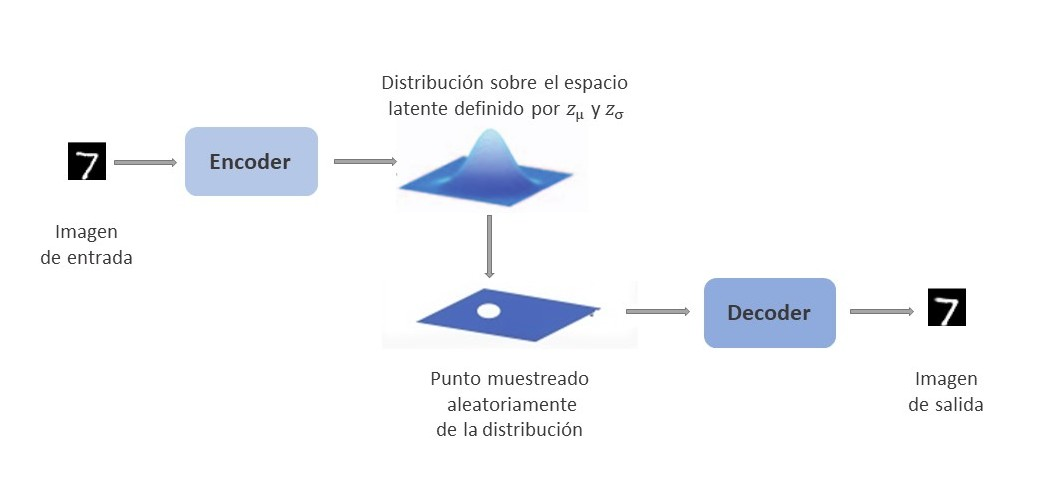
\includegraphics[width=5in]{Graphics/VAEMnist.JPG}
	
	\caption{ \small{Ejemplo de VAE transformando una imagen a 2 vectores, $z_{\mu}$ y $z_{\sigma}$, los cuales definen  una distribución de probabilidad sobre el espacio latente y son usados para generar un punto que será decodificado posteriormente.}}
	
	\label{VAEminist}
	
\end{figure}

En el aprendizaje automático, para lograr cierto nivel de inferencia, interesa encontrar la probabilidad conjunta entre la entrada $x$ y la variable latente $z$, denotada como $P_{\theta}(x, z)$ \cite{Advanced}. Las variables latentes no son parte del conjunto de entrenamiento pero recopilan ciertas propiedades observables en los datos. Luego $P_{\theta}(x)$ puede ser calculada como la distribución marginal: 
\begin{equation}
	P_{\theta}(x) = \int P_{\theta}(x, z)dz
	\label{eq:px}
\end{equation}

Al tratar de resolver la ecuación \ref{eq:px} se presenta el problema de que $P_{\theta}(x)$ no posee una forma analítica o un estimador eficiente. No puede ser diferenciable con respecto a sus parámetros \cite{Advanced} y, por tanto, el cálculo del gradiente como parte del algoritmo de descenso del gradiente no sería posible. En consecuencia, la optimización o proceso de \textit{backpropagation} en la red neuronal no tiene sentido. \cite{Chollet}.
%Chollet /113

Usando el teorema de Bayes se tiene una alternativa para la expresión en \ref{eq:px}:
\begin{equation}
	P_{\theta}(x) = \int P_{\theta}(x|z)P(z)dz.
	\label{eq:pxBayes}
\end{equation}

$P(z)$ es una distribución de probabilidad sobre $z$, no está condicionada a ninguna de las observaciones. 
%Si $z$ es discreto y $P_{\theta(x|z)}$ es una distribución Normal, entonces $P_{\theta}(x)$ es una mezcla de funciones Normales. Si $z$ es continuo, $P_{\theta}(x)$ es una mezcla infinita de Normales.

En la práctica, al intentar construir una red neuronal para aproximar $P_{\theta(x|z)}$ sin una función de pérdida adecuada, simplemente ignorará $z$ y llegará a una solución trivial \cite{Advanced} definida como:
\begin{equation*}
	P_{\theta(x|z)} = P_{\theta}(x).
\end{equation*}

Por lo tanto la ecuación \ref{eq:pxBayes} no proporciona una buena estimación de $P_{\theta}(x)$. En efecto, la ecuación \ref{eq:pxBayes} puede ser expresada también de la forma: 
\begin{equation}
	P_{\theta}(x) = \int P_{\theta}(z|x)P(x)dz .
\end{equation}

No obstante, sigue siendo intratable calcular $P_{\theta}(z|x)$. El objetivo de un VAE es encontrar una distribución que aproxime  $P_{\theta}(z|x)$ de la mejor manera posible. Para ello se centra en estimar la media y varianza correspondiente a dicha distribución. A continuación se exponen las ideas principales para lograrlo.

 
\subsection{Inferencia en el VAE}\label{3-VAEInference}
Con el propósito de obtener $P_{\theta}(z|x)$, el VAE introduce un modelo de inferencia variacional( \textit{encoder}):
\begin{equation}
	Q_{\phi}(z|x) \approx P_{\theta}(z|x).
\end{equation}

$Q_{\phi}(z|x)$ puede aproximarse por una red neuronal profunda mediante la optimización de los parámetros $\phi$. De esta manera, proporciona un buen estimador de $P_{\theta}(z|x)$; que además de ser parametrizable, es tratable su cálculo en términos computacionales. 

A partir del esquema de la figura \ref{AEdiagram}, se considera a $Q_{\phi}$ para inferir las posibles variables ocultas que se usan en la generación de los vectores latentes. Tal modelo se construye mediante una arquitectura de redes neuronales donde el modelo \textit{encoder} aprende una función de transformación  de $x$ a $z$ y de igual forma el \textit{decoder} de $z$ a $x$ como se visualiza en la figura \ref{VAEQPDistrib}.

%poner foto de https://www.jeremyjordan.me/variational-autoencoders/
\begin{figure}[!h]
	\centering
	
	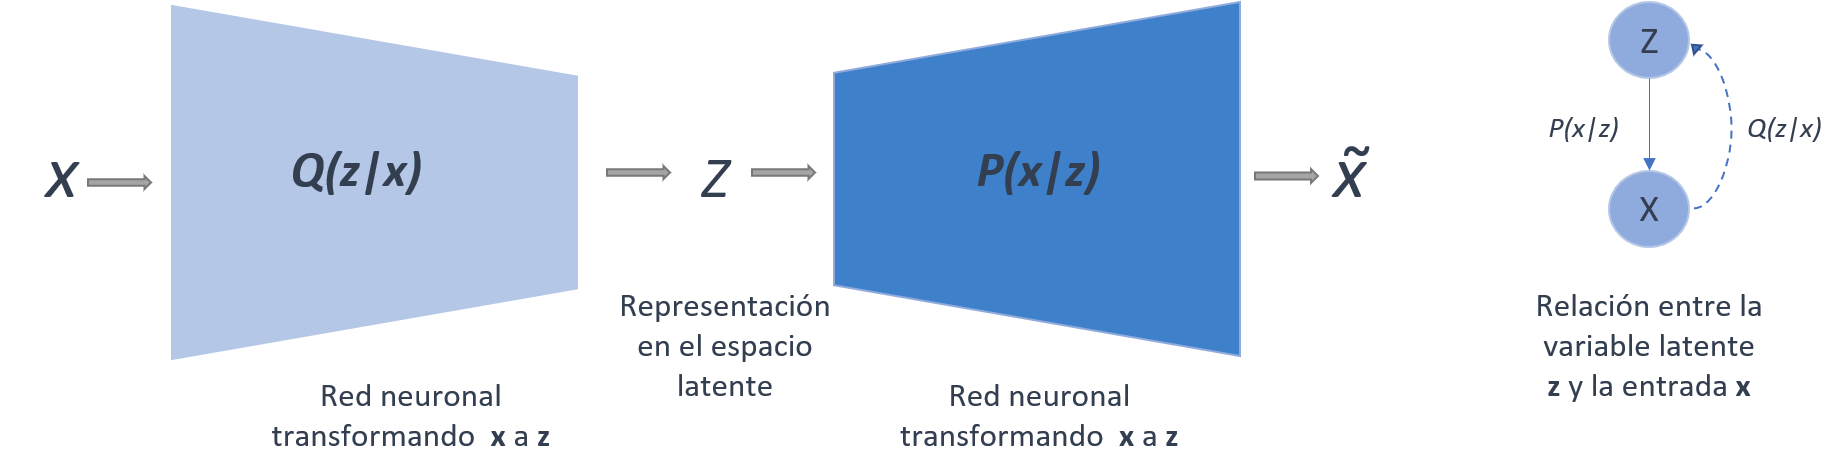
\includegraphics[width=5in]{Graphics/VAEQPDistribution.png}
	
	\caption{ \small{Representación del VAE mediante modelos neuronales}}
	
	\label{VAEQPDistrib}
	
\end{figure}


$Q_{\phi}(z|x)$ se distingue por ser una distribución gaussiana multivariada \footnote{En probabilidad y estadística, una distribución gaussiana multivariada, es una generalización de la distribución normal unidimensional a dimensiones superiores}. 
\begin{equation}
	Q_{\phi}(z|x) = \mathcal{N}(z; \mu(x), \sigma(x)*I)
\end{equation}

Tanto la media $\mu(x)$ como la desviación estandar $\sigma(x)$, se calculan por el modelo neuronal \textit{encoder} usando los datos de entrada. Para construir un verdadero modelo gaussiano multivariado, sería necesario definir una matriz de covarianza que describe la correlación entre las dimensiones. Sin embargo, los VAE evitan describir explícitamente las dependencias entre las dimensiones de z \cite{VAETutorial}. Adoptan un enfoque para lidiar con este problema: asumen que no hay una interpretación simple de las dimensiones de $z$, y en su lugar afirman que se pueden extraer muestras de $z$ de una distribución simple, es decir, $\mathcal{N}(0, I)$, donde $I$ es la matriz identidad.

%Sin embargo, el modelo se simplifica para que la matriz solo tenga valores distintos de cero en la diagonal, permitiendo describir esta información en un vector. La matriz diagonal implica que los elementos $z$ son independientes.

El modelo de inferencia $Q_{\phi}(z|x)$ genera un vector latente z a partir de la entrada $x$. $Q_{\phi}(z|x)$ juega el papel del \textit{encoder} en un modelo \textit{autoencoder}. Por otro lado, $P_{\theta}(z|x)$ reconstruye la entrada a partir de $z$. $P_{\theta}(z|x)$ actúa como el \textit{decoder} en \textit{autoencoder}. Para estimar $P_{\theta}(x)$, se debe identificar su relación con $Q_{\phi}(z|x)$ y $P_{\theta}(z|x)$. 

Como $Q_{\phi}(z|x)$ es un estimador de $P_{\theta}(z|x)$, la distancia entre ambas densidades condicionales se determina mediante la divergencia Kullback-Leibler (KL). Esta métrica es una medida no simétrica de similitud o diferencia entre dos funciones de distribución de probabilidad y en este caso se define como:

\begin{equation}
	D_{KL} (Q_{\phi}(z|x) \parallel P_{\theta}(z|x)) = \mathbb{E}_{z \sim Q} \left [ log Q_{\phi}(z|x) - P_{\theta}(z|x) \right ]
\end{equation}

La función de pérdida para este modelo consta de dos términos, uno que penaliza el error de reconstrucción (intuitivamente es quien maximiza la probabilidad de reconstrucción) y un segundo término que impulsa a la  distribución aprendida $Q_{\phi}(z|x)$ ser similar a la verdadera distribución  $P_\theta(z)$. Esta última se asume que sigue una distribución gaussiana para cada elemento $j$ del espacio latente. Luego, la función de pérdida final resulta en:

\begin{equation}
\mathcal{L'} = \mathcal{L}(x, \tilde{x}) + \sum_{j} KL(Q_{\phi}(z|x) \parallel P_{\theta}(z|x))
\end{equation}


Técnicamente el funcionamiento de un VAE consiste en:
\begin{enumerate}
	\label{VAESteps}
	\item La red \textit{encoder} transforma los datos de entrada $x$ en dos parámetros que se denotan como $z_{mean}$ y $ z_{log {\_} sigma} $ correspondientes a los valores $\mu$ y la $\sigma$ de la distribución Normal.
	
	\item Aleatoriamente se muestrea un punto $z$ de la distribución Normal asumida mediante:  
	\begin{equation}
	z = z_{mean} + exp(z_{log{\_}sigma})*\epsilon
	\end{equation}
	donde $\epsilon$ es un vector aleatorio de valores muy pequeños.
	
	\item La red \textit{decoder} convierte el punto $z$ al vector de entrada original.  
\end{enumerate}

Como $\epsilon$ es aleatorio, el proceso asegura que cada punto cercano al vector latente $z$ pueda ser decodificado a un vector similar a $x$. El hecho anterior asegura que el espacio latente sea continuo, así refiere \textit{Chollet et al} \cite{Chollet}. 

%Como se mencionó en \ref{3-VAEInference}, los parámetros del modelo se entrenan por medio de dos funciones de pérdida: la pérdida de reconstrucción que obliga a los vectores de salida coincidir con la entrada inicial y la divergencia KL entre la distribución latente aprendida y la verdadera distribución de probabilidad, actuando como término de regularización. Es decir, el VAE se entrena utilizando una función de pérdida personalizada debido a la penalización añadida, resultando en la suma de un término de reconstrucción y otro de regularización.
 
En esencia, la red \textit{encoder} (también conocida como red de inferencia \cite{BengioGood} ) se usa para describir una distribución de probabilidad de los elementos del espacio latente. Luego, al tomar muestras de este espacio, el \textit{decoder} se usa para formar un modelo generativo capaz de crear nuevos datos similares a los que se observaron durante el entrenamiento. En la siguiente sección, se presentan ejemplos de situaciones donde se aplican los VAEs para obtener una representación latente de cierta información.


\subsection{Aplicación de los VAEs a problemas similares}

Una de las aplicaciones más recientes de los VAEs en general, que comparte ideas con este trabajo es \cite{TrajectoryCompres}. Rákos et al. aborda el problema de comprimir trayectorias de vehículos del mundo real. Presentan un \textit{variational autoencoder} para codificar la información referente a las trayectorias. 

Durante el entrenamiento, el modelo aprende a codificar y decodificar estos datos y produce un pequeño vector de contexto de pocos elementos que puede representar el comportamiento del vehículo de manera probabilística. Muestran que la representación aprendida durante la compresión separa las trayectorias de acuerdo con tres clases de maniobra (mantenimiento de carril, cambio de carril derecho o cambio de carril izquierdo), evidenciando con ello gran capacidad para tareas de clasificación. 

 La propuesta parte de la hipótesis de predecir el vector de contexto de la trayectoria en lugar de la trayectoria en sí, pero se ve limitada por la carencia de un conjunto de datos de mayor dimensión y que represente mejor la dinámica y condiciones del ambiente de los vehículos. Aunque el sentido de estas trayectorias no comparte relación con las rutas del VRP, la idea detrás de la codificación mediante un \textit{variational autoencoders} sí lo hace.



%Los problemas de enrutamiento son especialmente significativos en gran variedad de aplicaciones modernas, como por ejemplo en la planificación de rutas, mantenimiento de redes, desarrollo de sistemas nanoelectrónicos de alto rendimiento, entre otros; y además, están caracterizados por datos esparsidos y no balanceados.

En \cite{VAESparseData} se manifiesta el problema de enrutar billones de componentes en dispositivos nanoelectrónicos. El proceso de enrutamiento en este tipo de sistema tiene en cuenta las componentes lógicas y las restricciones entre ellas como por ejemplo, la disposición vertical y horizontal de los cables físicos que las conectan. La solución brindada en este trabajo recibe una imagen como entrada, representada por un vector de píxeles de dimensión $nxn$ para un $n$ grande. En ella están comprendidas las características y restricciones del problema. La salida es un conjunto de posiciones que deben ser incluidas en las rutas contenidas en la imagen de entrada. 

Con el fin de maximizar la rutabilidad (cantidad de caminos generados) y minimizar la longitud del cable (cantidad de posiciones que ocupa un camino) en un espacio en \textit{2D} restringido, Utyamishev et al. \cite{VAESparseData} explota un proceso de entrenamientos progresivos del VAE para aprender una representación latente con datos altamente dispersos y no balanceados. Para cada ruta, el número de posiciones incluidos es $O(n)$, siendo significativamente menor que el número total de posiciones $n^2$. Esto último arroja datos dispersos y no equilibrados.

La noción de progresividad está dada porque el VAE fue diseñado para utilizar diferentes tamaños del conjunto de entrenamiento de forma incremental. Dicho método exhibe una rápida convergencia y alto grado de rutabilidad.

El trabajo presentado en \textit{Hottung et al.} \cite{HottungBT21} en mayo de 2021 aporta interesantes ideas para el desarrollo de esta tesis. Ofrecen un enfoque de optimización basado en aprendizaje que permite guiar la búsqueda dentro de la distribución de soluciones de alta calidad para una instancia del problema. Construyen un \textit{Conditional Variational Autoencoders} para transformar soluciones del problema de enrutamiento a puntos de un espacio continuo que, en conjunto, conforman un espacio de búsqueda. Su idea es que a partir de una solución buena $s$ y una instancia del problema $l$, codificar esta información a un vector $z$. Posteriormente la capa de decodificación unido a un algoritmo de optimización, en este caso con una estrategia de evolución diferencial, generan una nueva solución $s'$ a partir de $z$ y $l$. En esta propuesta se emplean técnicas de aprendizaje automático como los modelos \textit{sequence-to-sequence}, \textit{Pointer Networks}, \textit{attention mechanism} los cuales serán abordados en las próximas secciones, y por otra parte, el uso de métodos de optimización para la búsqueda en el espacio aprendido. 



%La investigación expone dos objetivos principales. Primeramente evidencian la efectividad del VAE como herramienta para representar trayectorias de vehículos de carretera en un vector de contexto denso y altamente comprimido. En segundo lugar, debido a la naturaleza de codificación continua del VAE, la codificación de similares trayectorias también están próximas entre sí en el vector de contexto, por lo que puede proporcionar la clase de maniobra a ejecutar sin información relativa al entrenamiento.



\section{Arquitecturas Sequence-to-Sequence}\label{2-Seq2seq}
Una solución a un problema de enrutamiento como el TSP y VRP puede ser interpretada, en su versión más simple, como un conjunto de listas de clientes donde cada lista representa una ruta. La disposición de los clientes dentro de la ruta es un factor determinante en el orden de los recorridos que se deben realizar. Por tanto, una solución se compone de un conjunto de rutas y estas a su vez, constituyen \textbf{secuencias} de clientes. Como parte de la revisión bibliográfica realizada se decidió indagar en los modelos \textit{sequence-to-sequence}, que pertenecen a la familia de modelos de aprendizaje automático para el procesamiento del lenguaje.

Los modelos \textit{sequence-to-sequence} \cite{SutskeverSeq2seqNN, PointerNVinyals} han resultado útiles en tareas donde se requiere convertir de una secuencia a otra. Han sido ampliamente estudiados en el campo de la traducción automática en los últimos 5 años, con el objetivo de traducir una secuencia en un determinado lenguaje a su secuencia correspondiente en otro lenguaje. La arquitectura general es muy parecida a un \textit{autoencoder}, pues consiste en dos redes neuronales recurrentes (RNN) nombradas \textit{encoder} y \textit{decoder}. La red \textit{encoder} lee la secuencia de entrada y encapsula la información extraída en un vector de tamaño fijo (o una secuencia de vectores); luego, el \textit{decoder} convierte la información codificada a una secuencia de salida. 

\subsection{RNN Encoder-Decoder}
Esta arquitectura que sirve como base y guía para los modelos \textit{encoder-decoders} de secuencias, está compuesto por un \textit{encoder} que lee la secuencia de entrada $X = (x_1, ..., x_T)$ y la convierte a un vector $c$. Cada elemento $x_i$ de $X$ se conoce también como palabra. La mayoría de las propuestas utilizan una RNN tal que: 
\begin{eqnarray*}
	h_t & = & f(x_t, h_{t-1}) \\
	c & = & q({h_1, ..., h_T})
\end{eqnarray*}
donde $h_t$ es el estado oculto de la RNN en el paso $t$, y $c$ es un vector de contexto generado a partir de la secuencia de estados ocultos. $f$ y $q$ son funciones no lineales, generalmente un caso de redes neuronales recurrentes nombradas como  \textit{LSTM} (Long Short-Term Memory).

El \textit{decoder} se entrena para predecir la próxima palabra $y_{t}$ dado el vector de contexto $c$ y todas las palabras predichas anteriormente $\{ y_1, ..., y_{t^{'} - 1}\}$. La unión secuencial de los $y_t$ conforman la predicción final $y$ que se define a través de la probabilidad condicional conjunta:
\begin{equation}
	p(y) = \Pi_{t=1}^{T}p(y_t| \{y_1, ..., y_{t-1}\}, c).
\end{equation}

Con una \textit{RNN} cada probabilidad condicional se modela como:
\begin{equation}
	p(y_t| \{y_1, ..., y_{t-1}\}, c) = g(y_{t-1}, s_t, c),
\end{equation}
donde $g$ es una función no lineal que estima la probabilidad de $y_t$, y $s_t$ es el estado oculto de la \textit{RNN}

En la arquitectura elemental Sequence-to-Sequence \cite{SutskeverSeq2seqNN}, la secuencia de entrada aparece solo una vez en el \textit{encoder} y la salida del mismo se genera a partir de un único vector (por ejemplo, el último estado oculto del \textit{encoder RNN}). Otras extensiones como \textit{Bahdanau et al.} \cite{BahdanauAlignTrans}, ilustran que la información de entrada se puede usar de forma más explícita para aumentar la cantidad de información durante los pasos de decodificación. Para ello, emplean otra red neuronal denominada mecanismo de atención (\textit{attention mechanism}) que $"atiende"$ todos los estados del \textit{encoder RNN}.

La idea detrás del mecanismo de atención es permitir que el \textit{decoder} se enfoque o preste atención en zonas importantes de la secuencia de entrada y use la información relevante para producir mejores secuencias de salida. El concepto de \textit{attention} ha sido usado por varios investigadores  \cite{PointerNVinyals, NazariRL, SetAE, OrderMatters} desde su introducción en 2015 por \textit{Bahdanau et al.} \cite{BahdanauAlignTrans}. \\

 \textit{ Bello et al.} \cite{bello2016neural} ofrece una propuesta sustentada en estos modelos, para predecir la distribución sobre las permutaciones de clientes en las soluciones del TSP. El análisis secuencial de las soluciones del VRP podría aportar resultados interesantes para la codificación de las mismas. Varias de las propuestas basadas en esta arquitectura, combinan también técnicas de aprendizaje reforzado. En la siguiente sección se abordan algunos ejemplos de aplicaciones de estos métodos a problemas de enrutamiento. 
 
 
\section{Reinforcement learning en problemas de enrutamiento.}\label{2-RL} 
Debido a su complejidad y naturaleza combinatoria, el VRP y sus variantes han sido candidatos naturales para problemas de optimización resueltos por métodos de ML. Por sus características secuenciales de decidir en qué orden se deben visitar los clientes, la dinámica del tiempo de demanda, y la falta de una distribución probabilística detrás de las rutas, estos métodos se basan principalmente en técnicas de aprendizaje reforzado (\textit{reinforcement , RL}).

La mayoría de los enfoques de RL para resolver el VRP, lo interpretan como un proceso de decisión de Markov, en el cual la solución óptima puede verse como una secuencia de acciones que deciden qué cliente visitar una vez ha sido atendido el cliente anterior. Estos algoritmos se enfrentan a dos dificultades principales. Primero, el VRP es un problema altamente combinatorio: codificar y decodificar el estado actual y la acción son un paso crucial. En segundo lugar, su estado se ve afectado por cada decisión, de modo que la representación del problema evolucione con el tiempo. Debido a estos inconvenientes, gran parte de los autores que se mencionan en este trabajo se han concentrado en modelos basados en la información del estado previamente observado. 

\textit{Vinyals et al}. \cite{PointerNVinyals} fueron los primeros en introducir las \textit{Pointer Networks}, un modelo inspirado en la arquitectura \textit{sequence-to-sequence}. 
%Estas redes se aplican a problemas de optimización combinatoria, donde la longitud de la secuencia de salida está determinada por la longitud de las secuencias de entrada.
 La arquitectura aprende la probabilidad condicional de una secuencia de salida formada por valores discretos que se corresponden a las posiciones de los elementos en la secuencia de entrada. Los autores entrenan su modelo para resolver instancias del TSP de hasta 50 clientes, usando un mecanismo de atención para obtener una permutación de la secuencia de entrada que constituye una ruta para el TSP. Durante la inferencia, seleccionar la secuencia con mayor probabilidad entre todas los opciones posibles es computacionalmente costoso e impracticable. Por ello se realiza un procedimiento de \textit{beam search} para encontrar la mejor secuencia posible. \textit{Beam search } es un algoritmo de búsqueda heurística que explora un grafo al expandir los $k$ nodos más prometedores dentro de un conjunto limitado de candidatos \cite{PeterNorvig}.
 
 Compararon el rendimiento con otros tres algoritmos, mejorando los resultados de \cite{SubOptTSPSolver} en casi todos los casos, excepto para instancias del problema con 40 clientes. En general mostraron buenos resultados para instancias de hasta 30 clientes.

Mientras que en \cite{PointerNVinyals} se obtiene una solución del TSP de una forma supervisada, \textit{Bello et al.} \cite{BelloNCORL} lo extiende con un aprendizaje no supervisado que emplea un método \textit{critic actor}. Este  método consiste en dos redes donde una actúa como actor y la otra como crítico. El actor decide qué acción se debe tomar y el cŕitico informa al actor qué tan buena fue la ación y cómo debe ejecutarla. 
%/315 	Advance  
Aplican una función de penalidad a partir de la distancia total recorrida en cada estado. Además, adaptaron su trabajo para hacer frente a las limitaciones del VRP, usando un término de alta penalidad sobre las soluciones no factibles. 

 \textit{Nazari et al.}\cite{NazariRL} amplía aún más este último para resolver el VRP, reemplazando la \textit{Pointer Networks} por un \textit{decoder RNN} basado en una proceso de \textit{attention}. Con ello logran capturar las dependencias de tiempo y los cambios del ambiente en el VRP, principalmente cómo evoluciona la demanda con el tiempo. Su modelo es invariante en el orden de la entrada (el orden de los clientes) por tanto puede manejar eficientemente elementos dinámicos en la entrada (por ejemplo, modificación de la demanda de un cliente una vez que este se visite). Obtienen resultados similares a las propuestas de última generación en problemas de pequeña y mediana dimensión. Múltiples extensiones se han introducido para resolver variantes del VRP, como \cite{VeraHVRP, ChenHVRP} para el HVRP, y \cite{ZhangWVRP} para el VRPTW. 

%Otra alternativa a las \textit{Pointer Networks} son los \textit{graph encoding}, los cuales manifiestan mejor la naturaleza combinatoria del problema que los modelos \textit{sequence-to-sequence}. En \textit{Khalil et al.} \cite{KhaliGraph} codifican las instancias usando un grafo constituido mediante una red neuronal, siendo así invariante en el orden de los nodos. Posteriormente ellos lo resuelven a través de un algoritmo de aprendizaje profundo \text{Q-learning} \cite{MnihQLearning}.

\textit{Hottung et al.} \cite{NeuralLargeHottung} propone un nuevo enfoque llamado \textit{neural large neigborhood search} (NLNS) que integra aprendizaje de heurísticas a la metaheurística de alto nivel \textit{large neigborhood search} (LNS). El mecanismo de aprendizaje está basado en una red neuronal profunda con un \textit{attention mechanism} cuyo funcionamiento consiste en aprender heurísticas para reparar soluciones incompletas del VRP y emplearlas después como guía en la búsqueda de nuevas soluciones. \\






























